%!TEX program = lualatex
\documentclass[12pt, a4paper]{article}
\usepackage[czech]{babel}
\title{The Gevo Times}

%Packages
\usepackage[dvipsnames]{xcolor}

%\usepackage[grid, gridunit=mm, gridcolor=blue!40, subgridcolor=blue!20]{eso-pic}

%Mřížka 

\usepackage[utf8]{inputenc}
\usepackage{amsmath}
\usepackage{amsfonts}
\usepackage{amssymb}

\usepackage[a4paper,includeheadfoot,margin=1cm]{geometry}


\usepackage{multicol}

\usepackage{tikz}
\usetikzlibrary{positioning}

%\usepackage{showframe}
%

\usepackage{graphicx}

\usepackage{wrapfig}

\usepackage{float}

\usepackage{url}

\usepackage[pdfpagemode=FullScreen, colorlinks=false]{hyperref}

\usepackage{anyfontsize}

\usepackage{emoji}


\usepackage[labelformat=empty]{caption}
\usepackage{qrcode}

%Defining things
\definecolor{gray}{rgb}{0.4,0.4,0.4}

%Header
\usepackage{fancyhdr}
\pagestyle{fancy}


\lhead{
	\footnotesize \thepage.
	}
\chead{
	\textbf{
		{\fontsize{45}{54}\selectfont The GEVO Times}
		}
	}

\rhead{
	\footnotesize Únor 2023 %\\[-1\baselineskip] 
	}

\lfoot{
    \begin{tikzpicture}[remember picture,overlay]
        \node [yshift=7mm, xshift=-89mm] (qro) at (current page.south){\qrcode[hyperlink,height=0.45in]{https://gevotimes.gevo.cz/}};
        \node [right=-2mm of qro](aaaa)
            {\emoji{mag-right}}
            ;
    \end{tikzpicture}
	  }
\cfoot{ \footnotesize
	Veškerý obsah najdete na webových stránkách gevotimes.gevo.cz \\
	Na Facebooku jsme jako The GEVO Times a na Instagramu jako @gevotimes \\
	Grafika a rozvržení: Eric Dusart
	}
\rfoot{\footnotesize
\begin{tikzpicture}[remember picture,overlay]
    \node [yshift=7mm, xshift=89mm] (qr) at (current page.south){\qrcode[hyperlink,height=0.45in]{https://forms.gle/gCsuqUS92MpSMiT16}};
    \node [left=-1mm of qr](aaa)
        {\emoji{writing-hand}}
        ;
\end{tikzpicture}


	}
\renewcommand{\headrulewidth}{0pt}
\renewcommand{\footrulewidth}{0.4pt}	% bar on bottom of page

\begin{document}

\sffamily

	\begin{tikzpicture}[remember picture,overlay]
        \node [yshift=0mm] (logo) at (current page.north)
            {\color{gray} \rule{\linewidth}{0pt}};
        \node [below=20mm of logo](first)
            {\color{gray} \rule{\linewidth}{1pt}}
            ;
		\node [below=-2mm of first](second)
		{\color{black} \rule{\linewidth}{3pt}}
		;
		\node [below=-2mm of second](third)
		{\color{gray} \rule{\linewidth}{1pt}}
		;
    \end{tikzpicture}

    \setlength{\columnsep}{30pt}
    \begin{multicols*}{2}
        \setlength{\columnseprule}{1pt}
        \begin{center}\section*{Praha a sníh}\end{center}

        Sníh jsem nikdy moc v lásce neměla. Zimu vlastně celkově nemám ráda, je hrozný chlad, mokro a člověk musí nosit tisíc vrstev, aby neumrzl. Jako právě já teď. Zachumlaná v dvou svetrech, kabátu a ještě v šále zrovna procházím kolem Staroměstského náměstí~a~sníh mi křupe pod nohama. Všude kolem jsou vánoční ozdoby a stánky s horkým svařákem~a~dalšími dobrotami. I když bych teď dala cokoliv za horké pití, z těch lidí všude mi naskakuje husina. Nikdy jsem nebyla přímo fanoušek trhů a dnešek není výjimkou. Výhled to je hezký, to uznávám. V podvečerním přítmí s jemným svitem lamp vypadají malé sněhové vločky padající z nebe opravdu kouzelně. Posadím se na lavičku~a~tiše vydechnu. Proč vlastně zimu tolik nesnáším? Asi za to taky může moje nechuť k Vánocům a všeho toho cirkusu okolo, ale jak tu tak sedím a~pozoruji padající vločky, říkám si, že bych možná tomuhle všemu měla dát druhou šanci. Že to možná není tak špatné, jak si myslím. Oči mi zabloudí zpět k vánočním trhům na náměstí. Pár minut se sama se sebou hádám, jestli to je dobrý nápad, nebo úplná blbost. Pravda je, že ten svařák bych si ale fakt dala. Nakonec to vzdám a s drobným úsměvem na rtech se rozejdu směrem ke stánkům.
        %\vspace*{-0.5\baselineskip}
        \begin{flushright}
			\footnotesize 
            Alžběta Špinarová
		\end{flushright}

        \begin{center}\section*{Soutěž o nejhezčí třídu s~Vánoční tématikou}\end{center}

        Týden před Vánoci u nás na škole proběhla soutěž o nejhezčí třídu. Odborná porota ze školního parlamentu prošla a hodnotila jednotlivé třídy. Kategorie hodnocení byly úklid, výzdoba (tématem byly Vánoce) a celkový dojem. Po vyhodnocení soutěž vyhrála 4.A. Děkujeme všem zúčastněným třídám a těšíme se na další soutěž a Vaši účast.

        \begin{flushright}
			\footnotesize 
            Adriana Fialková
		\end{flushright}

        \section*{Napište článek do Gevo Times}

        \hspace{\parindent} Stačí vyplnit jednoduchý formulář a my se Vám ozveme. Formulář najdete v QR kódu v pravém dolním rohu Gevo Times, na stránkách Gevo Times (QR kód vlevo dole) nebo na: \url{https://forms.gle/gCsuqUS92MpSMiT16}
        %107
        %\vfill\null
        %\columnbreak
        \begin{center}\section*{Vánoční koncert}\end{center}

        Jak všichni víte, 21. prosince 2022 se konal vánoční koncert. O písničkách, které tehdy zazněly, ví snad každý, každý je alespoň jednou slyšel. Mnoho lidí ale neví, jak koncert vznikal.

        Celý koncert se začal řešit lehce na poslední chvíli, základních příprav (námět, výběr písniček a~přibližný scénář) jsme se tehdy ujaly já (Agáta), Adri a~Kačka ze 4.A. Písničky byly téměř vybrány a odsouhlaseny paní profesorkou Vašátkovou, ale kdo je měl zpívat a~kdo hrát?

        Vydali jsme se tedy po celé škole, snažily se nalákat co nejvíce lidí do sboru a případně najít kandidáty do orchestru, chodily jsme do každé třídy, ale to vám nejspíš neuniklo. Přihlásilo se nám ve třídách celkem dost zájemců, ale druhý den na informační schůzku a na další zbývající schůzky, které se konaly mimo projektový týden, tolik lidí nedorazilo. Přesto jsme vytrvali a myslím, že to za to stálo.

        Náš projektový týden byl prodloužený a trval až do pátku. První den se nás setkalo najednou mnohem více a začalo se zkoušet naplno. Od rána do oběda jsme zpívali a snažili se naučit texty a výslovnost písniček v cizích jazycích. Naučit se texty zpaměti, to byl samozřejmě trošku problém, ale nakonec i ten se vyřešil.

        Bohužel, jak všichni víme, rozjela se všude chřipka a mnoho lidí ze sboru padlo s horečkou a kašlem. Všichni museli o to víc zatnout zuby a posílit své hlasy. Zda se nám to povedlo, můžete posoudit sami.

        Po projektovém týdnu nás stále čekalo pár zkoušek. Pak už následovala jen poslední, a to generální,~která se konala na místě, kde se pak odehrával koncert. Zkusili jsme si, jak zní sbor s mikrofony a~jak se rozléhají naše hlasy v kostelních prostorech. 
        
        Přišel konečný den, a to den koncertu. Ráno jsme se sešli na rychlou zkoušku a pak už následoval koncert pro Jižní Město; snad se nám povedl. Po chvilkové pauze následoval druhý koncert, a to pro Sázavskou.

        Nakonec je důležité říct, že náš koncert se nacvičil v plném počtu pořádně za sedm dní, a~děkujeme všem, kteří se do něj zapojili; a to učitelům i žákům, samozřejmě také divákům, kteří si snad náš koncert užili, ale hlavně paní profesorce Vašátkové.

\begin{flushright}
    \footnotesize 
    Agáta Pomahačová
\end{flushright}

    \end{multicols*}
    \newpage
    \begin{tikzpicture}[remember picture,overlay]
        \node [yshift=0mm] (logo) at (current page.north)
            {\color{gray} \rule{\linewidth}{0pt}};
        \node [below=20mm of logo](first)
            {\color{gray} \rule{\linewidth}{1pt}}
            ;
		\node [below=-2mm of first](second)
		{\color{black} \rule{\linewidth}{3pt}}
		;
		\node [below=-2mm of second](third)
		{\color{gray} \rule{\linewidth}{1pt}}
		;
    \end{tikzpicture}
    \begin{multicols*}{2}
        \setlength{\columnseprule}{1pt}
        \begin{center}\section*{Život za velkou louží}\end{center}

        Zdlouhavý proces plný nekonečného vyplňování dokumentů, psaní srovnávacích testů, předávání osobních údajů, nespočet telefonátů se zmateným koordinátorem zahraničních studentů, a nakonec nejméně dvacetinásobné podepsání prohlášení o tom, že skutečně nejsem prodejce drog, obchodník s lidským masem, terorista, či kterákoli nepříliš ideální varianta osoby hlásící se na střední školu v Americe. (Ne že by cokoli z toho bylo příliš vhodné v jakékoli jiné zemi…)  A pak najednou klika cvakla, dveře letí,~a já se vláčím s kufrem, o trojnásobné váze mně samotné, ze dveří. Tlumený šum letištní haly, pohled na rodiče vzdalující se za terminálem a v rozklepané ruce pas, studentské vízum, letenky a milion dalších papírů, bez kterých se můžu rovnou zabydlet na lavičce na jednom z gatů, protože mě nikdo nikam nepustí. A v pouhém mžiku oka už sedím v letadle, domov se mi na půl roku vzdaluje, a mně postupně těžkne hlava uvědoměním, jak nezvratné tohle všechno je.

        Takhle nějak začal můj studijní pobyt v Jižní Dakotě v polovině léta. Výběr státu proběhl až nepřirozeně náhodně a nenuceně. Jednoho dne jednoduše přišla moje teta a povídá: „nechceš do Dakoty?“ a~já jen pokrčila rameny a popravdě odvětila: „Tak jo,~hlavně když někam.“

        Jediný kritický bod nastal při hledání školy, která musela mít mezinárodní studentský program, aby mi na základě jejich dokladu o mém přijetí mohla americká ambasáda vydat studentské vízum. Člověk, co si studium zařizuje přes agenturu, tento problém pravděpodobně řešit nemusí, ale vzhledem k tomu, že já se vydala jinou cestou, musela jsem si splnit tato kritéria sama.

        Před odletem se musí ještě zařídit vyjádření praktického lékaře ke studentovu zdravotnímu stavu, fyzické kondici a případným alergiím. Věřím, že záleží na cílené destinaci, ale já musela navíc ještě vyplnit přibližně nekonečně stran dlouhý dotazník od americké ambasády, než se přesvědčili, že jsem skutečná žijící osoba s touhou po zahraničním studiu, a mohli mi vydat ono legendární vízum.

        Přestože příprava byla mnohdy náročná, místy až lehce vysilující, a začátky stresové, napjaté a vykročení z mé komfortní zóny dosáhlo úrovně, která se ani slovy nedá popsat, nepřeháním ani trochu, když řeknu, že to za to vše stálo.

        Tolik úžasných lidí, neuvěřitelných zážitků a nových zkušeností, které mě potkaly během jediného půlroku, mi už nikdy nikdo nevezme. Střet s novou kulturou, zemí, jazykem, přáteli, možnostmi a~mnohem dalšího. Nemohu samozřejmě s hlavou sebejistě vztyčenou hlásat, že všude to bude stejné, neboť z~velké části asi záleží na štěstí, ale mohu se radovat z toho,~že já ho měla, a pochybuji, že by pro mě celá situace mohla dopadnout lépe. I proto se nakonec z mého původního semestru stal celý rok a já se po dvou týdnech doma na Vánoce vracím opět za Atlantik,~přesvědčit se, že se mi to celé nezdálo.

        \begin{flushright}
			\footnotesize 
            Alžběta Mášková 
		\end{flushright}

        \begin{center}\section*{Filmové okénko}\end{center}

        Tento měsíc vychází třetí pokračování filmu Ant-Man, Ant-Man: Quantumania.
        Co víme: Na základě upoutávky promítané na SDCC 2022 můžeme udělat pár odhadů o zápletce filmu. Scott Lang (Paul Rudd) se těší své proslulosti jako jeden z hrdinů, kteří zachránili svět. Tato radost se však zmírní, když jeho dcera Cassie (Kathryn Newtonová) začne následovat jeho zločinecké stopy.
            
        Pro tento měsíc jsem vybrala knihu It Ends with Us (2016), která je v přípravách na zfilmování. Pro připravovaný film jsou zatím potvrzeni pouze dva herci: Blake Lively jako Lily Bloom a Justin Baldoni jako Ryle Kincaid. Zatím není žádné potvrzené datum vydání, ale můžeme očekávat uvedení filmu někdy v~roce 2024.

        \subsection*{Postava / herec měsíce}
        Pro postavu měsíce jsem si vybrala Yelenu Belovu, protože herečka Florence Pugh (27), která ji hraje, 
        \setlength{\intextsep}{0pt}
        \setlength{\columnsep}{12pt}
		\begin{wrapfigure}{r}{0.2\textwidth}
            %\vspace*{-12pt}
            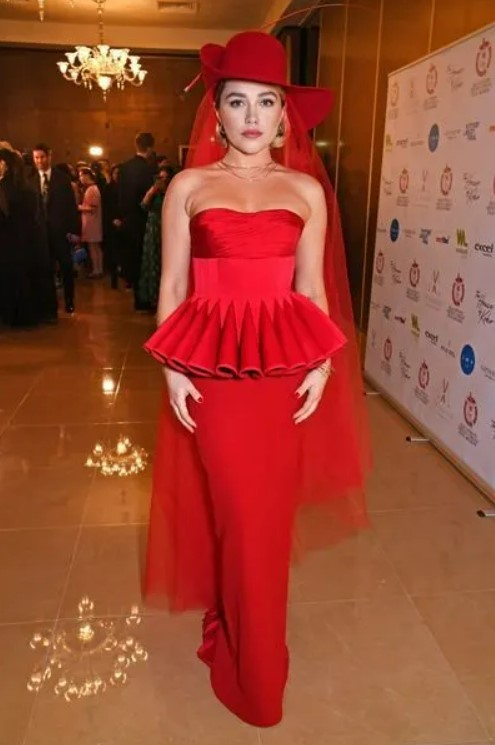
\includegraphics[width=0.2\textwidth]{1}
            \caption*{Florence Pugh}
        \end{wrapfigure}
        se v neděli 5. února zúčastnila předávání cen London Critics' Circle Film Awards v~The May Fair Hotel v~Londýně. Za svou práci ve filmech jako Don’t Worry Darling, The Wonder, Puss In Boots a The Last Wish byla oceněna cenou britsko-irská herečka roku.
        \begin{flushright}
			\footnotesize 
            Karolína Elisabeth Bednářová
		\end{flushright}



    \end{multicols*}

    

\end{document}